\documentclass[a4paper,10pt]{article}

\usepackage[usenames,dvipsnames]{color}
\usepackage{comment}
\usepackage[utf8]{inputenc}
\usepackage{listings}
\usepackage[pdfborder={0 0 0}]{hyperref}
\usepackage{amssymb}
\usepackage{amsmath}
\usepackage{float}
\usepackage{graphicx}

\graphicspath{{./images/}}

\definecolor{Gray}{gray}{0.5}
\definecolor{OliveGreen}{cmyk}{0.64,0,0.95,0.40}

\lstset{
    language=C++,
    basicstyle=\ttfamily,
    keywordstyle=\color{OliveGreen},
    commentstyle=\color{Gray},
    captionpos=b,
    breaklines=true,
    breakatwhitespace=false,
    showspaces=false,
    showtabs=false,
    numbers=left,
}

\title{
	An Efficient Parallel Signal Temporal Logic Implementation \\
    VU GPU Architectures \& Computing \\
    SS 2013
}

\author{
    Bernhard Denner,
    Jakob Gruber,
    Mino Sharkhawy
}

\renewcommand{\And}{\wedge}
\newcommand{\Or}{\vee}
\newcommand{\Neg}{\neg}
\newcommand{\Impl}{\rightarrow}
\newcommand{\Until}{\mathbf{U}}
\newcommand{\Evtl}{\diamondsuit}
\newcommand{\Alw}{\square}
\newcommand{\Buntil}{\mathbf{U}_I}
\newcommand{\Bevtl}{\diamondsuit_I}
\newcommand{\Balw}{\square_I}

\begin{document}

\begin{comment}
Problem statement, State of the art (semantics, ...), Sequential algorithms, Parallel ..., Test cases, benchmarks, How the project went, what we did.
\end{comment}

\maketitle
\pagebreak
\tableofcontents
\pagebreak

\section{Background}

Temporal logic describes a system of rules for representing and reasoning about propositions
qualified in terms of time\footnote{\url{http://en.wikipedia.org/wiki/Temporal_logic}}.
It consists of the usual logical operators $\And, \Or, \Neg, \Impl$ as well as
some collection of modal operators. In particular, signal temporal logic as used in this
project defines the following additional operators:

\begin{itemize}
\item $a \: \Until \: b$: The \textbf{UNTIL} operator is true if and only if $a$ is true
      at all points until some point at which $b$ becomes true.
\item $\Evtl \: a$: The \textbf{EVENTUALLY} operator is true iff a becomes true at any point
      in the future. It is equivalent to $\mathit{true} \: \Until \: a$.
\item $\Alw \: a$: The \textbf{ALWAYS} operator is true iff a is true at every point in the range.
      It is equivalent to $\neg \Evtl \neg a$.
\end{itemize}

Each of these three operators also has a bounded variant ($\Buntil, \: \Bevtl, \Balw$) which
for each point $a$ in the signal restricts the processed interval to $a + I$.

Furthermore, besides the usual boolean semantics (which always evaluate to either \textit{true} or
\textit{false}), signal temporal logic is also defined over real-valued quantitative semantics which
can be interpreted as indicating ``how much'' a condition is satisfied at any given point.

\section{State of the Art} \label{sec:stateoftheart}

A. Donze, T. Ferrere, O. Maler, \emph{Efficient Robust Monitoring for STL} describes
sequential algorithms calculating robustness signals for all STL operators within linear
time complexity.

Algorithms are provided for the $\And, \Neg, \Until, \Evtl, \Bevtl$ operators, which are then used
to construct all remaining operators as follows:

\begin{align}
a \Or b &= \Neg (\Neg a \And \Neg b) \\
a \: \Until_{[s, t]} \: b &= \Alw_{[0, s]} \And \Evtl_{[s, t]} \And \Evtl_{[s, s]} (a \: \Until \: b)\\
\Alw \:  a &= \Neg \Evtl  \Neg a \\
\Balw \: a &= \Neg \Bevtl \Neg a
\end{align}

Sequential implementations are outlined in the following sections. Each signal consists
of a sequence of \lstinline|sigpt_t| structs:

\begin{lstlisting}
typedef struct {
    float t;  /* The time. */
    float y;  /* The value. */
    float dy; /* The derivative. */
} sigpt_t;
\end{lstlisting}

\subsection{NOT}

The $\Neg$ operator simply negates all signals points.

\begin{figure}[H]
\begin{lstlisting}
Compute(NOT, y) {
    /* ny is the number of points in y. */
    for (i = 0; i < ny; i++) {
        result[i].y = -y[i].y;
    }
    return result;
}
\end{lstlisting}
\label{fig:not}
\caption{The NOT operator.}
\end{figure}

\subsection{AND}

The $\And$ operator basically performs a point-wise minimum between both incoming signals.
This is complicated by the fact that signal values need to be interpolated for all
cases in which contains time points not found in the other signal. Additionally,
all intersections between both signals must also be added to the result.

\begin{figure}[H]
\begin{lstlisting}
Compute(AND, x, y) {
    ts = /* union of all time points in x, y, and all intersections between them */;
    i = 0;
    for (t in ts) {
        result[i].t = t;
        result[i].y = min(
            interpolate(x at time t),
            interpolate(y at time t));
        i++;
    }
    return result;
}
\end{lstlisting}
\label{fig:and}
\caption{The AND operator.}
\end{figure}

\subsection{EVTL}

The sequential $\Evtl$ implementation is simply a reverse running maximum, again
complicated by the existence of intersections between the current running maximum
and the signal.

\begin{figure}[H]
\begin{lstlisting}
Compute(EVTL, y) {
    mx = y[ny - 1].y;
    result.push_front({ y[ny - 1].t, mx });

    for (i = ny - 2; i >= 0; i--) {
        if (y[i + 1].y < mx && y[i].y > mx) {
            t = /* Interpolate time of intersection */
            result.push_front({ t, mx });
        }
        mx = max(y[i].y, mx);
        result.push_front({ y[i].t, mx });
    }
    return result
}
\end{lstlisting}
\label{fig:evtl}
\caption{The EVTL operator.}
\end{figure}

\subsection{UNTIL}

$\Until$ is composed of several $\Evtl, \And$, and $\Neg$ operations performed on
individual segments. Note that \lstinline|z0| always references the value from the
previous iteration. This is also the only operator which actually uses the signal derivative
values \lstinline|signal.dy|.

\begin{figure}[H]
\begin{lstlisting}
Compute(UNTIL, x, y) {
    z0 = -INFINITY;
    for (i = nx - 1; i >= 0; i--) {
        if (x[i].dy <= 0) {
            z1 = Compute(EVTL, y);
            z2 = Compute(AND, z1, x);
            z3 = Compute(AND, const_signal(x[i + 1].y), z0);
        } else {
            z1 = Compute(AND, y, const_signal(x[i].y));
            z2 = Compute(EVTL, z1);
            z3 = Compute(AND, x, z0);
        }
        z4 = Compute(OR, z2, z3);
        result.push_front(/* All points in z4. */);
        z0 = const_signal(z4[0].y);
    }
    return result
}
\end{lstlisting}
\label{fig:until}
\caption{The UNTIL operator.}
\end{figure}

\subsection{BEVTL}

The $\Bevtl$ calculates the maximum of the window $t + I$ for each $t$. It is
essentially a running maximum of the entire signal with a window size of $b - a$,
where $I = [a,b]$. To do this, the sequential implementation iterates over the signal
and keeps a list of points, which still have to be considered for the current time.

You can see the algorithm in Listing~\ref{fig:bevtl}.

\begin{figure}[H]
\begin{lstlisting}
Compute(BEVTL, y, a, b) {
    ya = shift(Compute(EVTL, y), a);
    yb = shift(Compute(EVTL, y), b);
    yd = Compute(AND, ya, yb);
    s = y[0].t - b;
    t = s;
    i = 0;
    M = {};
    while (t + a < y[n - 1].t) {
        t = min(y[min(M)].t - a, y[i + 1].t - b);
        if (t == y[min(M)].t - a) {
            M.del(min(M));
            s = t;
        }
        if (t == y[i + 1].t - b) {
            while (y(y[i + 1].t - b) >= y(max(M)) && M != {}) {
                M.del(max(M));
            }
            M.add(i+1);
            i += 1;
        }
        if (s >= y[0].t) {
            if (M == {}) {
                z[s:t] = yd[s:t];
            } else {
                z[s:t] = Compute(OR, yd[s:t], y[min(M)]);
            }
        }
    }
    return z;
}
\end{lstlisting}
\label{fig:bevtl}
\caption{The BEVTL operator.}
\end{figure}

\section{Problem Statement}

The algorithms shown in section \ref{sec:stateoftheart} all have linear complexity
but are completely sequential.
GPUs offer the potential for vast performance improvements, but require algorithms
which are suited to their highly parallel architectures. The objective of this project
was to attempt to parallelize all algorithms required for STL processing. In case of success, these could then be

\begin{itemize}
\item benchmarked and compared to the existing Breach\footnote{\url{http://www.eecs.berkeley.edu/~donze/breach_page.html}} implementation,
\item swapped into Breach to replace the sequential algorithms, and
\item integrated with a parser in order to process entire STL formulas.
\end{itemize}

\section{Implementation}

The following sections provide an in-depth examination of our implementation
as well as related tools and test methods.

\subsection{Tools}

The target platform for this project was the parallel programming and computing platform CUDA\footnote{\url{http://www.nvidia.com/object/cuda_home_new.html}}.
We also made heavy use of the parallel algorithms library Thrust \footnote{\url{http://code.google.com/p/thrust/}}, mainly for standard algorithms such as parallel merges, and prefix sums.

This project was mostly written in C++ together with a mix of C, Bash (for our test scripts), and MATLAB (interaction with Breach and test generation).

Expected test case results as well as benchmark traces were generated by Breach (rev 452) as well as MATLAB R2013a.

We tested on several different systems with varying GPUs and CUDA versions, but
our main test machine used CUDA 5.0 V0.2.12211. The minimal tested compute capability
was 1.2.

Our build system was CMake\footnote{\url{http://cmake.org/}} 2.8.7, integrated with the
C unit testing framework Check\footnote{\url{http://check.sourceforge.net/}} 0.9.8.

\subsection{Test Environment}

Our test environment used a combination of GNU Make, CTest (which is a part of CMake), and Check to automate testing at the end of each build.

Each operator had its own test suite, which in turn contained a sanity test (to ensure that the operator actually managed to run without crashing) as well as
several tests comparing the output of our GPU operator implementations to the
corresponding Breach operators.

Care had to be taken to account for acceptable signal deviations such as additional
interpolated points (one or more points located within a straight line segment).

Input signals as well as expected outputs were generated by MATLAB scripts (located
in the \verb|matlab/| folder).

% TODO: Possibly fill this in?
% \subsection{Breach Integration}

\subsection{Parallel Algorithms}

\subsubsection{NOT}

The parallel NOT operator does exactly the same thing as the sequential one. It
schedules the entire signal to multiple processors on the GPU which in turn negate
the set of points they have been assigned.

\subsubsection{Consolidate}
\label{sec:consolidate}

\begin{figure}[H]
\begin{lstlisting}
void
consolidate(const thrust::device_ptr<sigpt_t> &lhs,
            const int nlhs,
            const thrust::device_ptr<sigpt_t> &rhs,
            const int nrhs,
            thrust::device_ptr<sigpt_t> *olhs,
            thrust::device_ptr<sigpt_t> *orhs,
            int *nout);
\end{lstlisting}
\caption{
\label{fig:parallel_consolidate}
The consolidate interface.}
\end{figure}

Given two incoming signals $lhs, rhs$, \lstinline|consolidate| builds a
merged time sequence which contains all time points as well as all intersection
time points of both signals. The resulting time sequence is used to reconstruct
the these signals using interpolation. This operation is trivial as a sequential
operation, but quite involved when done in parallel.

The first part of our algorithm is concerned with associating each point $l \in lhs$
with a point $r \in rhs$ such that $r$ is the latest point in $rhs$ with $r.t \leq l.t$. Likewise, each point $r \in rhs$ must be associated with a point $l \in lhs$.

\begin{lstlisting}
t1 = merge lhs and rhs time sequences;

t1lhs = extract all lhs times from t1
t1lhs = inclusive_scan(t1lhs, max)
/* t1lhs now contains the associated lhs point for each index. */

t1rhs = extract all rhs times from t1
t1rhs = inclusive_scan(t1rhs, max)

t1 = add the information from t1lhs and t1rhs to t1

t1 = remove duplicate time points from t1
\end{lstlisting}

Using the associations determined in the previous section we can easily calculate
all intersections without losing performance by searching for associated points
in the opposing signal.

\begin{lstlisting}
t2 = a new signal twice as long as t1, t2[i * 2] = t1[i]
/* All t2[i * 2 + 1] points are potential intersections. */

t2 = calculate_intersections(t2)

t2 = remove potential intersections which did not turn out to be an intersection
\end{lstlisting}

Finally, the resulting time sequence is then used to create the outgoing signals
$lhs', rhs'$ by interpolating the incoming signals.

\begin{lstlisting}
(clhs, crhs) = extrapolate(lhs, rhs, t2)
return (clhs, crhs)
\end{lstlisting}

\subsubsection{AND}

\begin{figure}[H]
\begin{lstlisting}
void
stl_and(const thrust::device_ptr<sigpt_t> &lhs,
        const int nlhs,
        const thrust::device_ptr<sigpt_t> &rhs,
        const int nrhs,
        thrust::device_ptr<sigpt_t> *out,
        int *nout)
{
	consolidate(lhs, rhs, clhs, crhs);
	return pairwise_minimum(clhs, crhs);
}
\end{lstlisting}
\caption{
\label{fig:parallel_and}
The parallel AND operator interface and high-level implementation.}
\end{figure}

Interface and a high-level implementation overview of the AND operator can be found 
in figure \ref{fig:parallel_and}.

The entire complexity of the AND operator is hidden in the fact that
both signals may not have the same set time points, and that new points
may be generated through intersections between the two.

The \lstinline|consolidate()|
function takes two such signals $lhs, rhs$, and returns equivalent signals $lhs', rhs'$ which include
all of these additional points. The set of time points in $lhs'$ is equal to the set
of time points in $rhs'$.

All that remains is to build the point-wise minimum over both signals, which
can be easily done completely in parallel.

\subsubsection{EVTL}

\begin{figure}[H]
\begin{lstlisting}
void
stl_evtl(const thrust::device_ptr<sigpt_t> &in,
         const int nin,
         thrust::device_ptr<sigpt_t> *out,
         int *nout);
\end{lstlisting}
\caption{
\label{fig:parallel_evtl}
The EVTL interface.}
\end{figure}

The parallel EVTL first calculates for every point $t$ the maximum of all points from
$t$ to the end of the signal. It uses a scan for this operation. After this step the
EVTL for each point in the input signal is already correct.

However, in the case that the EVTL value rose in an earlier point (i.e.
\lstinline|Compute(EVTL, y)[i].y > Compute(EVTL, y)[i+1].y|), the exact point in time,
where the EVTL is greater than \lstinline|Compute(EVTL, y)[i+1]| for the first time
has to be calculated in order to generate a valid signal.

Since this operation only needs values at $i$ and $i + 1$ and doesn't depend on the
output anywhere else, it can be performed for each pair of points independently.

\begin{figure}[H]
\begin{lstlisting}
Compute(EVTL, y) {
    z = scan(y, max_y);

    /* Each iteration of this loop can be scheduled to a different GPU processor. */
    for (i = 0; i < ny; i++) {
        if (i < ny - 1 && z[i].y > z[i + 1].y) {
            newp.t = intersect(z[i], y[i], z[i + 1], y[i + 1]);
            newp.y = z[i + 1].y;
            z.insertAfter(i, newp);
        }
    }

    return z;
}

max_y(a, b) {
    ret.t = b.t;
    ret.y = max(a.y, b.y);

    return ret;
}
\end{lstlisting}
\label{fig:par_evtl}
\caption{The parallel EVTL operator.}
\end{figure}

\subsubsection{UNTIL}

While we were unable to completely parallelize the UNTIL operator due to the fact,
that each iteration of the loop in the sequential operation (see
Listing~\ref{fig:until}) depends on the previous result, we could extract large parts
of said loop and parallelize these.

Specifically, the computation of all points in $z1$, $z2$, $z3$ and $z4$ can be
parallelized. The $z0$ is computed sequentially on the CPU.

\begin{figure}[H]
\begin{lstlisting}
void
stl_until(const thrust::device_ptr<sigpt_t> &lhs,
          const int nlhs,
          const thrust::device_ptr<sigpt_t> &rhs,
          const int nrhs,
          thrust::device_ptr<sigpt_t> *out,
          int *nout);
\end{lstlisting}
\caption{
\label{fig:parallel_until}
The UNTIL interface.}
\end{figure}

For the two given signals $lhs$ and $rhs$, we calculate $lhs \Until rhs$.

\begin{lstlisting}

clhs;
crhs;
nc;

consolidate(lhs, nlhs, rhs, nrhs, &clhs, &crhs, &nc);

\end{lstlisting}

First, the two signals are consolidated such that each one contains all points in
time of both signals and their intersections (see Section~\ref{sec:consolidate}).

\begin{lstlisting}

neg_dys_lhs;
neg_dys_rhs;
pos_dys_lhs;
pos_dys_rhs;

clhsi = intervals(clhs);
crhsi = intervals(crhs);

split_by_dy(clhsi, crhsi, nc, &neg_dys_lhs, &neg_dys_rhs, &pos_dys_lhs, &pos_dys_rhs, (<= 0));

\end{lstlisting}

Next the signals are split according to the $dy$ value in $clhs$. The points in
$crhs$ and $clhs$ where it is $\leq 0$ end up in $neg\_dys\_lhs$ and $neg\_dys\_rhs$,
while the other end up in $pos\_dys\_lhs$ and $pos\_dys\_rhs$ respectively.

Additionally, for each of these points at index $i$ the interval from this point to
the one at $i+1$ is calculated.

\begin{lstlisting}

iz1 = for_each_interval(Compute(EVTL), neg_dys_rhs);
iz2 = for_each_interval(Compute(AND), iz1, neg_dys_lhs);

ez1 = for_each_interval(Compute(AND), neg_dys_rhs, constant(pos_dys_lhs));
ez2 = for_each_interval(Compute(EVTL), ez1);

\end{lstlisting}

Then we calculate the $z1$ and $z2$ from for all iterations where $dy \leq 0$ and for
all iterations where $dy > 0$ in parallel.

\begin{lstlisting}

z2 = merge(iz2, ez2);
z0 = seq_z0(clhs, crhs, z2, nc);

/* This is the LHS for our z3 calculation. */
z4 = extract_z4(clhs);

z3 = for_each_interval(Compute(AND), z4, z0);
resulti = for_each_interval(Compute(OR), z2, z2);

\end{lstlisting}

As stated above, we have to compute $z0$ sequentially. This is done in exactly the
same way as shown in Listing~\ref{fig:until}. The calculation takes place on a single
device thread; experimental results have shown that the overhead produced by
copying device segments from the device to the host (and back again) far outweighs
the time gained by utilizing the faster host CPU.

With the $z0$, we can then calculate the $z3$ and our result in parallel.

\begin{lstlisting}

*out = merge_intervals(resulti);
*nout = out.n;

\end{lstlisting}

Lastly, the intervals in $result$ are merged into one final signal.

\subsubsection{BEVTL}

The sequential BEVTL algorithm uses an efficient running maximum calculation to
achieve linear time complexity. Adapting this running maximum for parallel execution
turned out to be infeasible as it would have quadratic space complexity.

The current parallel BEVTL algorithm has thus a run time complexity of $O(f(n,p,w))$,
where $w$ is the size of the window used.

While the breach reference implementation uses every point $t$ from the original
signal as the starting point of a window and then stores the maximum over that window
at the point $t - s$, the parallel implementation stores the maximum for the window
starting at $t + s$ at $t$. This leads to the two implementations generating disjoint
result signals. However, the values the parallel implementation calculates are
correct.

The primary reason not to perform the BEVTL the same way Breach does is that we
initially assumed, that the start and end points of a signal do not change. This
calculation would have violated this assumption and would have required changes to
all operators.

\begin{figure}[H]
\begin{lstlisting}
void
stl_bevtl(const thrust::device_ptr<sigpt_t> &in,
          const int nin,
          const float s,
          const float t,
          thrust::device_ptr<sigpt_t> *out,
          int *nout);
\end{lstlisting}
\caption{
\label{fig:parallel_bevtl}
The BEVTL interface.}
\end{figure}

For the given signal $in$, we calculate $\Bevtl in$, where $I = [s,t]$.

\begin{lstlisting}
start_points = calc_ofs_points(in, s);
end_points = calc_ofs_points(in, t);

all = merge(in, start_points, end_points);
all = unique(all);
\end{lstlisting}

The implementation first calculates the window start and end points and merges them
with the original signal, while eliminating all duplicate points.

\begin{lstlisting}

start_idx = get_ofs_idx(in, s, all);
end_idx = get_ofs_idx(in, t, all);

parallel for i in [0 .. in.length] {
    out[i] = max_from_to(start_idx[i], end_idx[i], all);
}

\end{lstlisting}

Then, for all points in $in$ the indices of the according window's start and end
points in $all$ are calculated. Lastly, for each point $i$ in $in$ the maximum of the
points between $start\_idx[i]$ and $end\_idx[i]$ in $all$ is calculated and stored in
$out[i]$. While the calculations for each point are performed in parallel, the
running time of each thread depends on the size of the window.

% Who did what? Challenges? ... ?

\section{Results}

The STL operators were parallelized with varying degrees of success:

As expected, parallelizing the NOT operator was trivial, with a resulting complexity of $O(\frac{n}{p})$. More surprisingly, all other
operators proved to be much more of a challenge than initially expected.

The AND and EVTL operators were also parallelized successfully, with a complexity only depending on $n$ and $p$.

The UNTIL algorithm was only partially parallelizable; in particular,
$z_0 = z_2 \Or (z_4 \And z_{0_{prev}})$ could not be solved with a single scan since
the operation is not associative. Another proposed solution, which worked by unrolling this formula over all points
and then running a segmented scan resulted in a space complexity which made processing even fairly small signals impossible within the constraints of current GPUs. We were also sceptical if such a solution could result in any speed-up over
the existing linear sequential algorithm. In the end, we compromised by performing
as much as we could in parallel, and calculating $z_0$ sequentially.

Finally, we implemented a parallel algorithm for the BEVTL operator. However,
our idea for creating and maintaining a bounded running maximum also proved to
be infeasable because of its space-complexity. Once again we had to compromise:
the current implementation is completely parallelized, but its complexity depends
on the window size (= the bounds) as well as the signal length.

% TODO: Say something about benchmark results either here or in the next section.

\subsection{Benchmarks}

The benchmarks were executed on host '{\it bellum}', provided by the institute. This machine is equipped with a {\it Intel Core2 Quad Q9550 @ 2.83GHz}, {\it 8GB RAM} and a {\it Nvidea GeForce GTX 670}. The {\it GeForce GTX 670} card has the following specification:

% TODO put this in a table
\begin{lstlisting}
  CUDA Driver Version / Runtime Version          5.5 / 5.0
  CUDA Capability Major/Minor version number:    3.0
  Total amount of global memory:                 4096 MBytes
  ( 7) Multiprocessors x (192) CUDA Cores/MP:    1344 CUDA Cores
  GPU Clock rate:                                980 MHz
  L2 Cache Size:                                 524288 bytes
  Total amount of constant memory:               65536 bytes
  Total amount of shared memory per block:       49152 bytes
  Total number of registers available per block: 65536
  Warp size:                                     32
\end{lstlisting}

Our code was compiled with and tested with the {\it CUDA Development Toolkit 5.0} (exact $nvcc$ version: {\it Cuda compilation tools, release 5.0, V0.2.1221}). This toolkit comes with a {\it Thrust version 1.5.3}.

For running the benchmarks we created test signals with matlab. We used two different signal types, with varying granularity, thus different amount of point per signal. 
The first signal type consist of two signals, which were used for testing binary operators ($AND$, $OR$, $UNTIL$). These signal pair (sig 1 and sig 2) was designed to generate a varying robustness signal for these operators.
These signals and the resulting signals for the $AND$ and $UNTIL$ operators are show in figure \ref{fig:sig1_sig2_and_until}
\begin{center}
    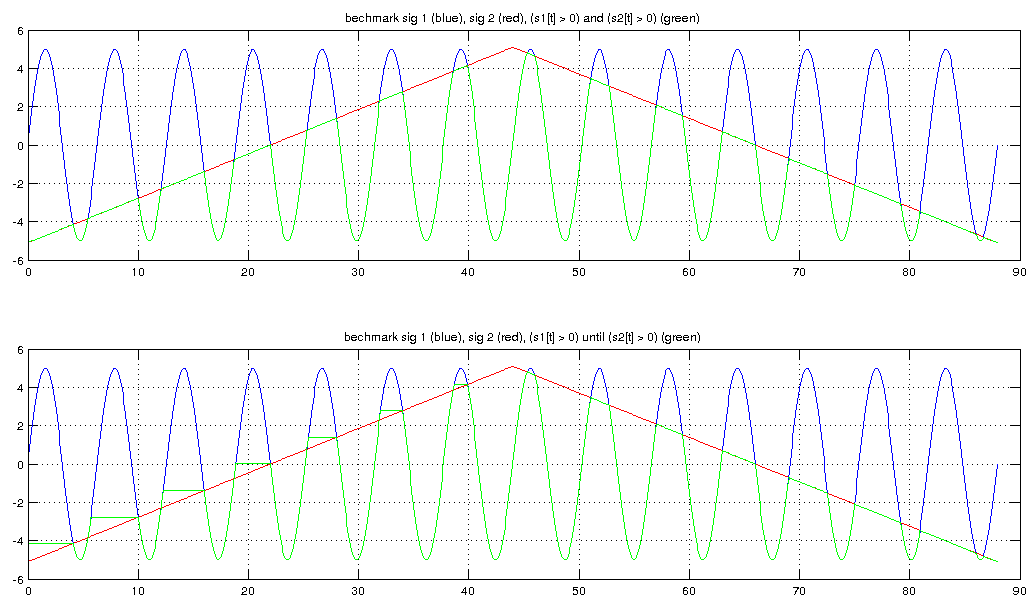
\includegraphics[scale=0.3]{bm_sig1_and_until.png}
%    \captionof{Benchmark signals: sig1, sig2, AND, UNTIL}
    \label{fig:sig1_sig2_and_until}
\end{center}    
The second signal type was used for testing unary operators, mainly $EVENTUALLY$ and $ALWAYS$. The decreasing amplitude of this signal ensures that the resulting robustness signals for these operators also vary as much as possible. This signal (sig 3) together with the resulting signals for $EVENTUALLY$ and $ALWAYS$ are shown in figure \ref{fig:sig3_evtl_alw}
\begin{center}
    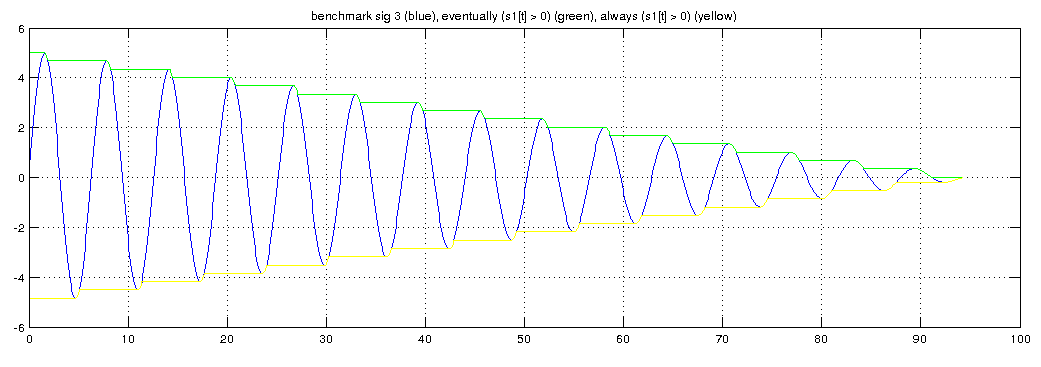
\includegraphics[scale=0.3]{bm_sig3_ev_alw.png}
%    \captionof{Benchmark signal: sig3, ALWAYS, EVENTUALLY}
    \label{fig:sig3_evtl_alw}
\end{center}

For our tests we used signals with 1.000, 10.000, 100.000, 1.000.000 and 5.000.000 points. Also some signal parameter where adjusted (e.g. the number of iterations...). 
Additionally to these benchmarks we created also test cases with random signals, thus signals with a defined number of points and random amplitude values. 

To distinguish easily between those test cases we introduced the following naming schema for test cases: test cases with defined signal types: $[operator name]-[number of points]$ and for the randomly generated test cases: $[operator name]-rand-[number of points]$.

The benchmarks where executed in the following way, which is implemented in the Bash script $matlab/run_benchmark.sh$:
\begin{itemize}
	\item generate signals with matlab 
	\item run Breach implementation on the signals
	\item write signals and Breach results to files
	\item run CUDA implementation with on the signals
	\item (optionally) do a compare of the resulting signal of CUDA implementation and Breach code
\end{itemize}

We tried to only measure the time of the robustness calculation. For the Breach implementation we used the $tic$, $toc$ functions from Matlab, directly before and after the calculation function. For our CUDA implementation we created a benchmark tool called $stl_bench$ which measures the elapsed time directly before and after the call to the calculation function, by using the CUDA Event functions.

To get more reliable results the robustness calculation code was executed ten times on the same signal and the mean value was used as resulting time.

% TODO: Test system specs, GPU, compiler version, benchmark mode (minimum of 10 runs),
% benchmarks for all basic operators (NOT,AND,EVTL,UNTIL,BEVTL), graphs (runtime / size)

\section{Further Work}

Plenty of work remains for future projects.

Completely and optimally parallelizing both the UNTIL and BEVTL operators still needs
to be investigated.

Room for improvement remains for optimizing all operators. For example, using streams
and optimizing memory allocation and deallocation immediately comes to mind.

An initial formula parser already exists. A future project could work on integrating the operator implementations with a component which operates on the abstract syntax tree produced by the parser to process complete formulas.

Likewise, the problem of arbitrary expressions ($\log(s_0) \; \text{UNTIL} \; \text{fft}(..)$) is also still unsolved.

Make operators scalable for multiple GPUs.

\end{document}
